\documentclass{article}

\title{Project 1 : Graphs and Network Flows}
\author{Aashith Kamath Manjeshwar, Daksha Asrani, Saikrishna Badrinarayanan}
\newcommand{\R}{\mathbf{R}}
\newcommand{\U}{\mathbf{U}}
\newcommand{\V}{\mathbf{V}}
\newcommand{\W}{\mathbf{W}}

\usepackage{graphicx}
\graphicspath{ {plots/} }
\begin{document}
\maketitle

In this project, we study two social networks -  facebook and google+. Each of them is modeled as a graph which 
denotes users' personal friendship network. We compute 
the community structure of these graphs and explore their applications. The project was coded in the language R.

\paragraph{Problem 1}: \\
In this problem, we first download the facebook graph edgelist and check if the graph is connected.
It turns out that the graph is indeed \textbf{connected}. The diameter of the network is \textbf{8}.

Next, we plot the degree distribution of the graph. The degree distribution is a plot containing the various degrees of the nodes 
in the graph on the x-axis and their corresponding density (frequency of that degree occuring divided by the total number of nodes) on the y-axis.\\

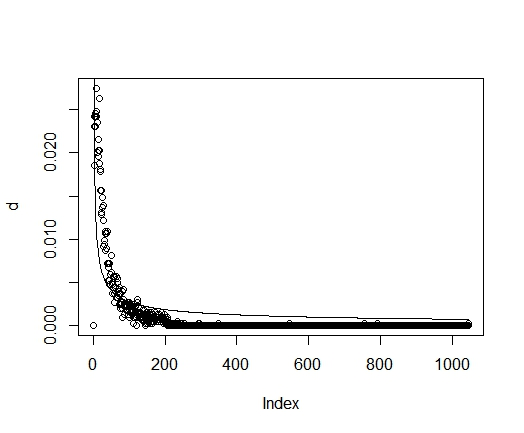
\includegraphics[scale=0.4]{ques1a} \\

We then try to fit a curve on this graph. This is done using non-linear square curve fitting by minimizing the total mean 
squared error. The reason being that the degree distribution plot looks like a power law curve and to 
find out the best power that fits the 
curve with minimal error we need a  
function that regresses to find the polynomial that fits the data with minimum error. The non-linear square curve
function performs exactly this.
The total mean squared error is $\mathbf{5.853918 * 10^{-06}}$.

Finally, we also find the average degree of the graph which is $\mathbf{0.0009560229}$\\

\hrule

\paragraph{Problem 2}:\\
We first create the personal network of the first node in the graph - i.e the node with id as $1$. The vertices in the personal network of the 
consist of all the neighbors of node 1 and itself. The edges of the personal network are created by 
including all edges in the original graph that have both ends within the personal network.
We note that all the nodes in the personal network share one common feature - in that, they all have at least one mutual friend, which is node 1. 
This is an important property of any personal network. We compute the number of nodes and edges in the personal network.
The number of nodes is $348$ and the number of edges is $2866$.
We also observe that the personal network is connected which follows from the fact that all of them have an edge to node 1 (the primary node 
based on which the personal network is created).\\

\hrule

\paragraph{Problem 3}:\\
We define core nodes to be nodes in the graph with more than 200 neighbours. We compute the number of 
core nodes to be $40$. The average degree of the core nodes is $279.375$.\\

We choose one core node (node with id = 1) and we find this core node's personal network. The notion of 
personal network has been defined in the previous question. The personal network is plotted below where we mark the 
core node in black.\\
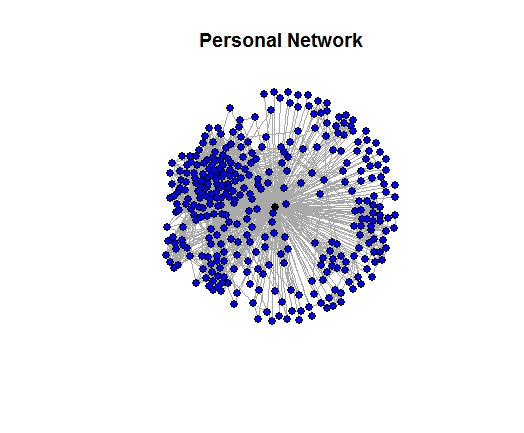
\includegraphics[scale=0.4]{q4b} \\

We then compute the personal network's community structure using 3 methods - fast greedy,  edge betweenness and 
infomap. We color each community differently in the plot to help identify them and to distinguish between the communities.
\begin{itemize}
	\item \textbf{Fast Greedy}\\
	When we use this method, the number of communities is $8$ and the modularity of the community
	structure is $0.4131$.
	In the first plot shown below, the x-axis denotes the sizes of the communities and the y-axis has the number of communities with that size.\\
	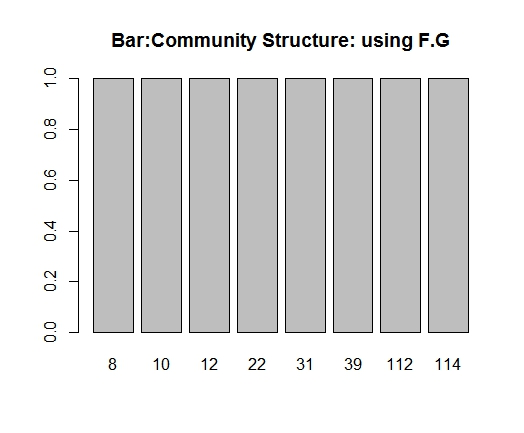
\includegraphics[scale=0.4]{q4a} \\
	In the next plot we provide a pictorial representation of the community structure.\\
	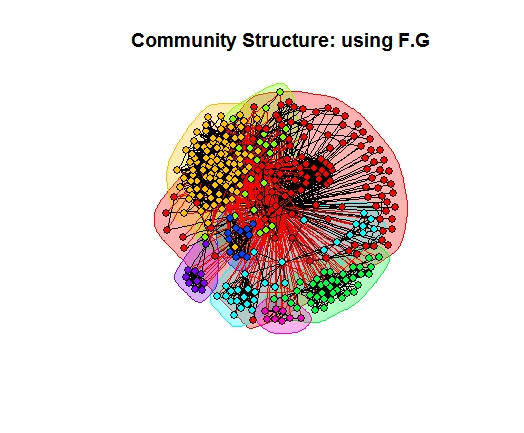
\includegraphics[scale=0.4]{q4c} \\ 
	\item \textbf{Edge Betweenness}\\
	When we use this method, the number of communities is $8$ and the modularity of the community
	structure is $0.3533$.
	In the first plot shown below, the x-axis denotes the sizes of the communities and the y-axis has the number of communities with that size.\\
	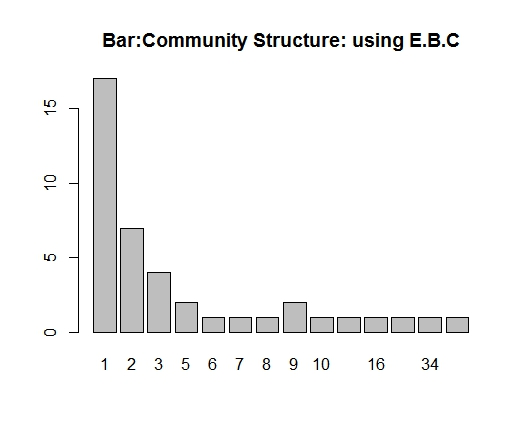
\includegraphics[scale=0.4]{q4d} \\
	In the next plot we provide a pictorial representation of the community structure.\\
	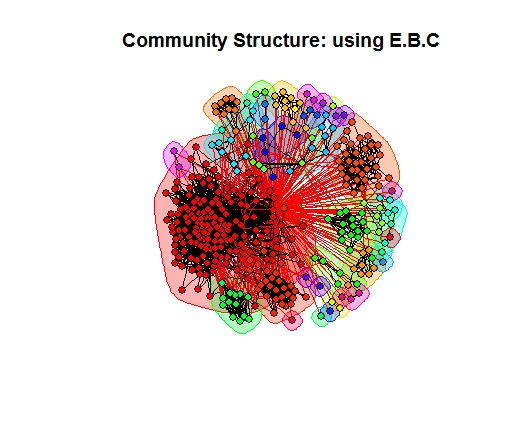
\includegraphics[scale=0.4]{q4e} \\ 
	\item \textbf{Infomap}\\
	When we use this method, the number of communities is $26$ and the modularity of the community
	structure is $0.3891$.
	In the first plot shown below, the x-axis denotes the sizes of the communities and the y-axis has the number of communities with that size.\\
	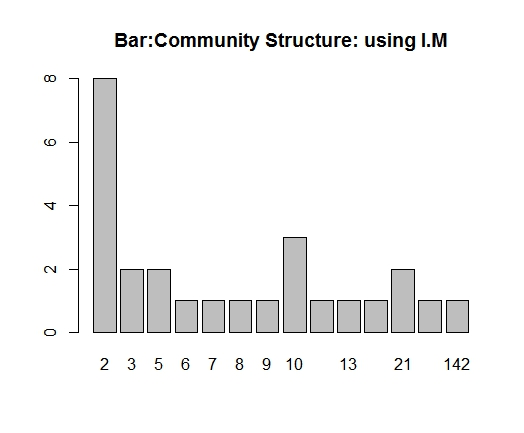
\includegraphics[scale=0.4]{q4f} \\
	In the next plot we provide a pictorial representation of the community structure.\\
	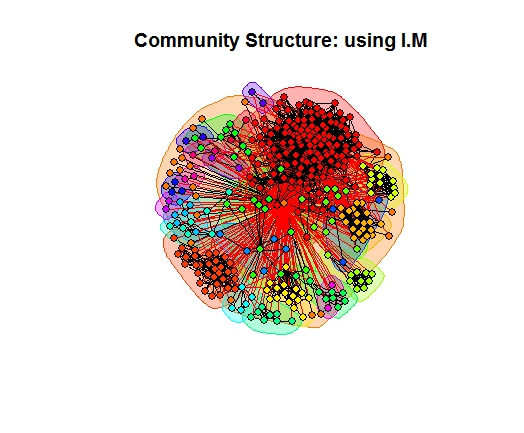
\includegraphics[scale=0.4]{q4g} \\ 
\end{itemize}
From the above plots, we observe that the community structures created using edge betweenness and infomap are very similar. This is 
noticed in the distribution of number of communities corresponding to a particular size - as seen in the first plot for each method. In both these methods, the number
of communities with small sizes is high and the count tapers off as the size of the community increases. However, in the fast greedy approach,
the number of communities is roughly the same for different sizes following no pattern like in the above cases. Also, the total number of communities
is much lesser in the case of fast greedy in comparison to the other two methods where they are roughly the same.  \\

\hrule

\paragraph{Problem 4}:\\
In this problem, we repeat the same procedure as in the previous question but with a small change - 
we remove the core node from the personal network and then perform the computation of the community structures.
First, here is the personal network after removing the core node :\\
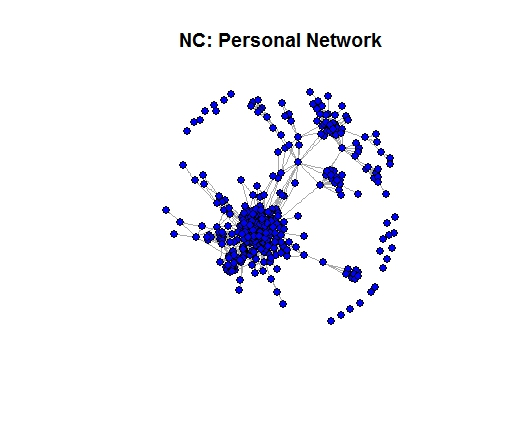
\includegraphics[scale=0.4]{q5b} \\

We then compute the personal network's community structure using 3 methods - fast greedy,  edge betweenness and 
infomap. We color each community differently in the plot to help identify them and to distinguish between the communities.
\begin{itemize}
	\item \textbf{Fast Greedy}\\
	When we use this method, the number of communities is $8$ and the modularity of the community
	structure is $0.4429$.
	In the first plot shown below, the x-axis denotes the sizes of the communities and the y-axis has the number of communities with that size.\\
	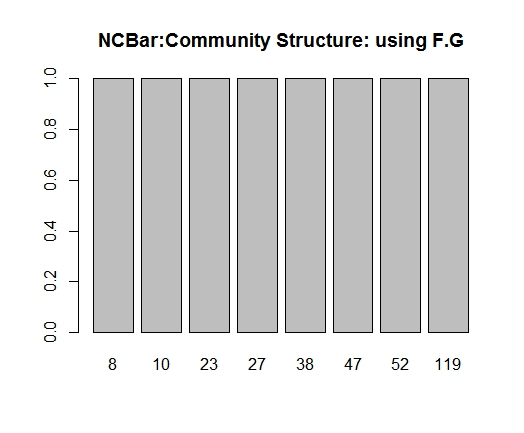
\includegraphics[scale=0.4]{q5a} \\
	In the next plot we provide a pictorial representation of the community structure.\\
	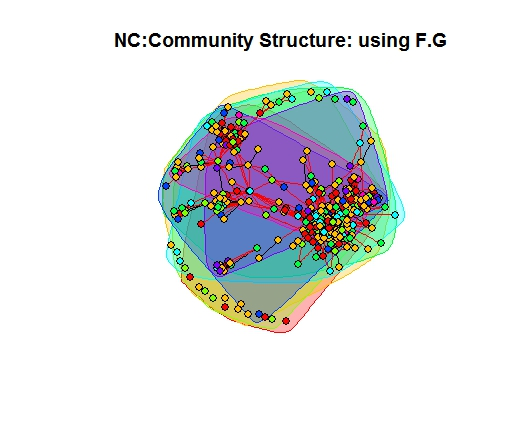
\includegraphics[scale=0.4]{q5c} \\ 
	\item \textbf{Edge Betweenness}\\
	When we use this method, the number of communities is $32$ and the modularity of the community
	structure is $0.4139$.
	In the first plot shown below, the x-axis denotes the sizes of the communities and the y-axis has the number of communities with that size.\\
	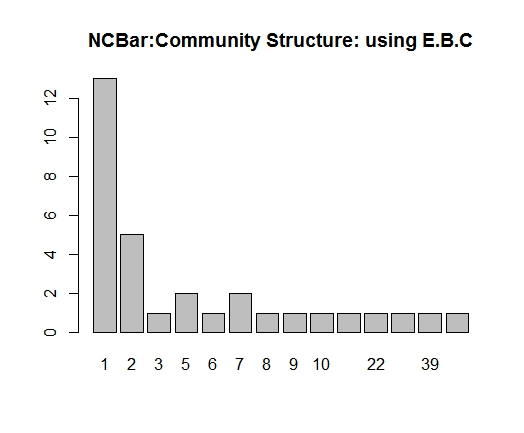
\includegraphics[scale=0.4]{q5d} \\
	In the next plot we provide a pictorial representation of the community structure.\\
	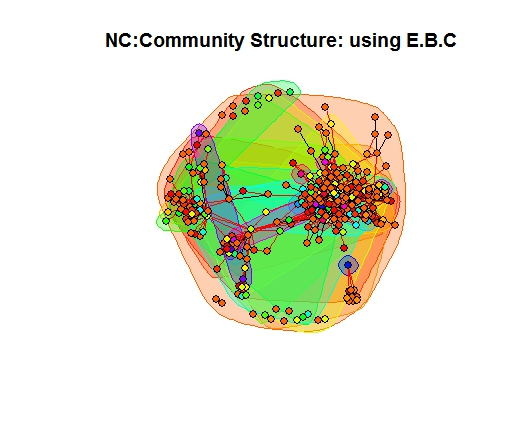
\includegraphics[scale=0.4]{q5e} \\ 
	\item \textbf{Infomap}\\
	When we use this method, the number of communities is $22$ and the modularity of the community
	structure is $0.4158$.
	In the first plot shown below, the x-axis denotes the sizes of the communities and the y-axis has the number of communities with that size.\\
	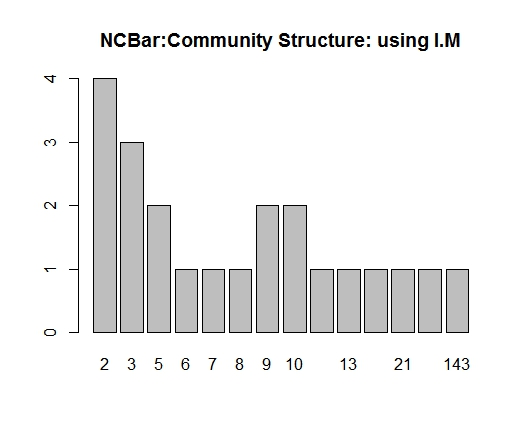
\includegraphics[scale=0.4]{q5f} \\
	In the next plot we provide a pictorial representation of the community structure.\\
	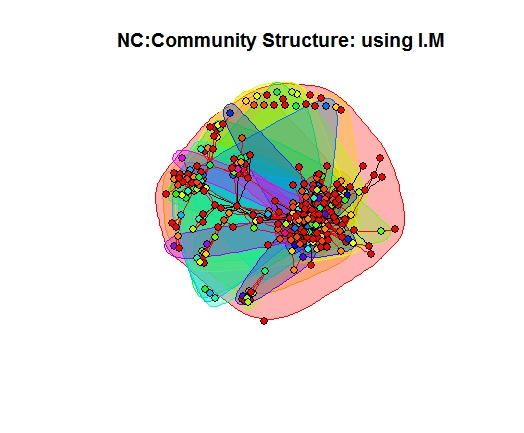
\includegraphics[scale=0.4]{q5g} \\ 
\end{itemize}
From the above plots, we observe that the community structures created using edge betweenness and infomap are very similar. This is 
noticed in the distribution of number of communities corresponding to a particular size - as seen in the first plot for each method. In both these methods, the number
of communities with small sizes is high and the count tapers off as the size of the community increases. However, in the fast greedy approach,
the number of communities is roughly the same for different sizes following no pattern like in the above cases. Also, the total number of communities
is much lesser in the case of fast greedy in comparison to the other two methods where they are roughly the same.  

\textbf{Key Observation}:\\
After removing the core node from the personal network, we observe an increase in the number of 
communities using all three algorithms for finding community structure of a graph. The modularity values 
also increase. This is because the personal network consists of all nodes connected to the core node, irrespective 
of whether the other nodes are connected or not. So, when the core node is removed from the personal network, the 
density of the subgraph decreases. This 
can be a probable cause for the increase in the number of communities.

\hrule

\paragraph{Problem 5}:\\
In this problem, we calculate the embeddedness and dispersion in the personal network of each core node. For 
a given node $x$, embeddedness is defined as the number of mutual friends of that node and the core node.
Dispersion is defined as the sum of distances between every pair of mutual friends of $x$ and the core node
calculated in a modified graph where we remove $x$ and the core node.
Here, the notion of distance is not definite. We explore two notions - the first one corresponds to the
standard notion of distance between any pair of vertices in a graph, which is the number of nodes in the shortest
path between the two vertices under consideration. Let's call the dispersions obtained by this method as 
dispersion 1.
For the next notion, we refer to ideas from the paper given in the reference section.
We choose the measure that works ``best'' for the problem addressed in that paper. Though that may not be the
best one in our case among the several approaches that they use, we stick to trying out just that one for now.
For a given node $x$ in the personal network of a core node $y$, this new distance 
between two nodes $a$ and $b$ (who are each mutual friends of $x$ and $y$) is defined to 
be 1 if $a$ and $b$ are not directly connected and they have no other mutual friend 
in the personal network other than $x$ and $y$. Let's call the dispersion obtained by this method as dispersion 2.\\

We compute the embeddedness and the two dispersion values for every node in every personal network.
Then, we plot a graph that contains the average embeddedness of each personal network (averaged over all nodes in the personal network)
on the y-axis and the corresponding personal network (indexed in some order) on the x-axis. Similarly, we plot average dispersion versus
personal network for both our dispersion measures. These plots are shown below.\\

\begin{enumerate}
 \item \textbf{Embeddedness}\\
 In the following histogram, the x-axis contains the average embeddedness values and the y-axis contains their
 frequency - that is, the number of personal networks whose average embeddedness is this.\\
 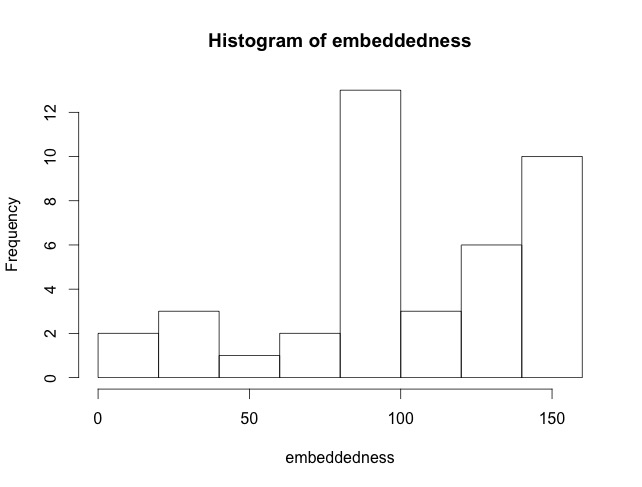
\includegraphics[scale=0.4]{5-a} \\
 Next, we plot a curve where the x-axis contains the personal networks and the y-axis contains the embeddedness
 values of the personal networks.\\
 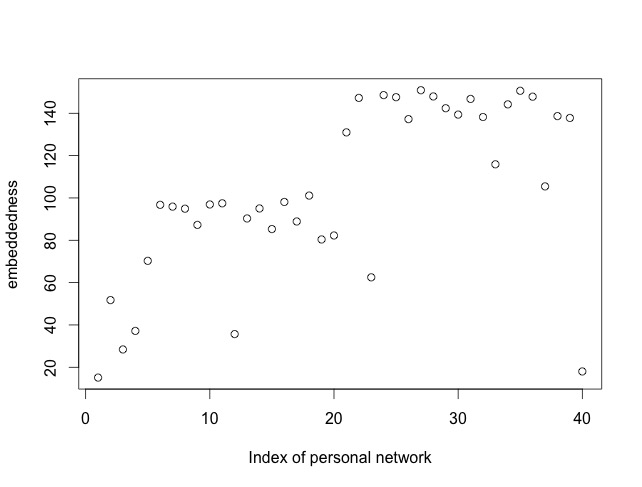
\includegraphics[scale=0.4]{5-b} \\
 
 \item \textbf{Dispersion-1}\\
 In the following histogram, the x-axis contains the average dispersion values and the y-axis contains their
 frequency - that is, the number of personal networks whose average dispersion is this.\\
 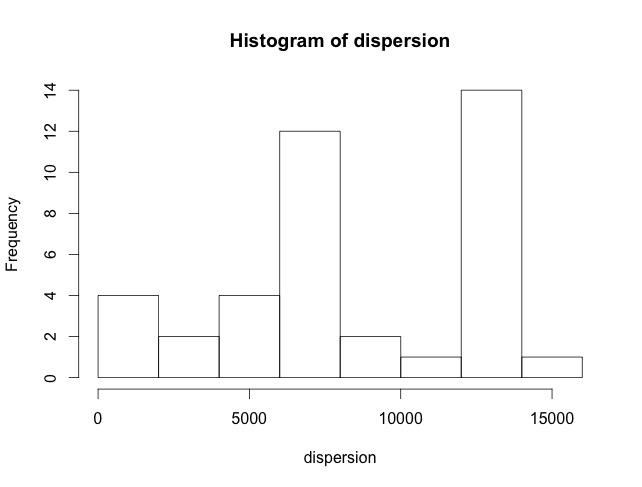
\includegraphics[scale=0.4]{5-c} \\
 Next, we plot a curve where the x-axis contains the personal networks and the y-axis contains the dispersion
 values of the personal networks.\\
 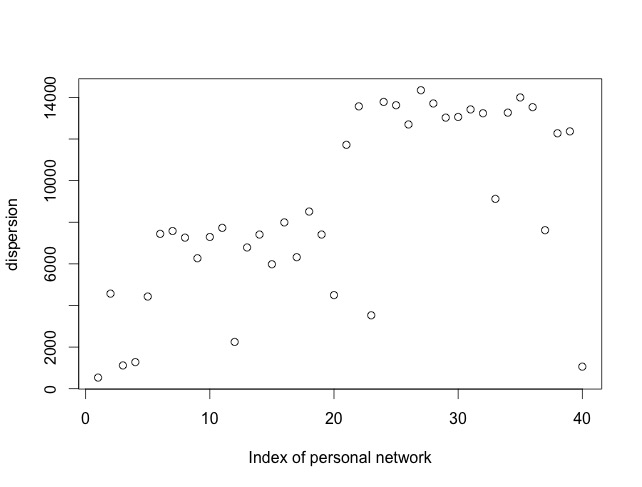
\includegraphics[scale=0.4]{5-d} \\

 \item \textbf{Dispersion-2}\\
 In the following histogram, the x-axis contains the average dispersion values and the y-axis contains their
 frequency - that is, the number of personal networks whose average dispersion is this.\\
 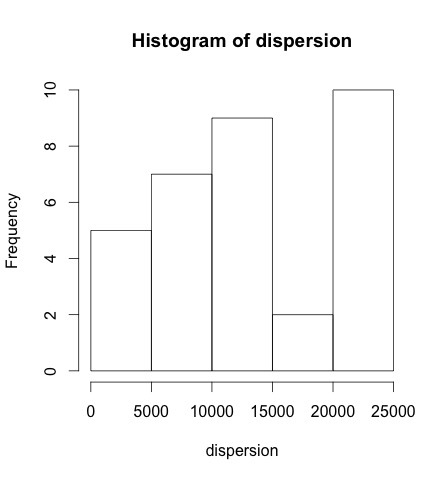
\includegraphics[scale=0.4]{5-e} \\
 Next, we plot a curve where the x-axis contains the personal networks and the y-axis contains the dispersion
 values of the personal networks.\\
 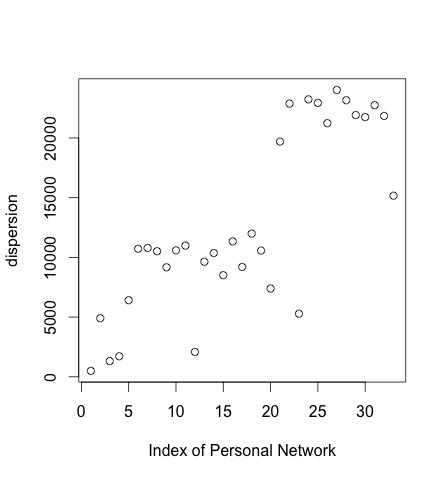
\includegraphics[scale=0.4]{5-f} \\
 
 \end{enumerate}
Next, we choose three personal networks and plot them along with their community structure using a separate colour for 
each community to distinguish between them. We highlight the nodes with the maximum dispersion, maximum embeddedness
and maximum ratio of dispersion to embeddedness in each network. We also highlight the edges incident to these nodes. We do this for both notions of dispersion. Thus, we have 
two plots per personal network.\\
\begin{enumerate}
 \item \textbf{Personal Network 1}\\
 The core node is node with id 1. The node with maximum embeddedness is 57.
 The node with maximum dispersion1 is 278 and the one with maximum dispersion2 is 57.
 The node with the maximum ratio of dispersion1 to embeddedness is 72.
 The node with the maximum ratio of dispersion2 to embeddedness is 34.\\
 \textbf{Using Dispersion 1 :}\\
 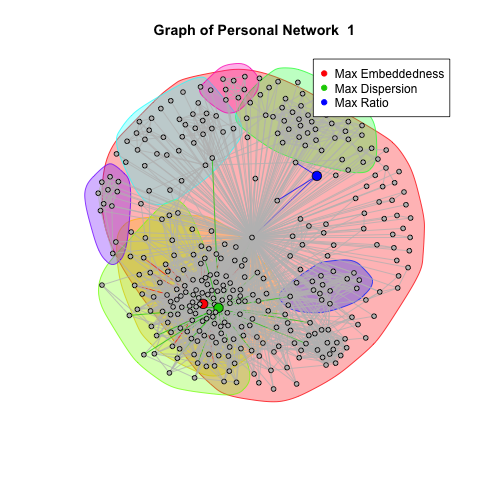
\includegraphics[scale=0.4]{d11} \\
 \textbf{Using Dispersion 2 :}\\
 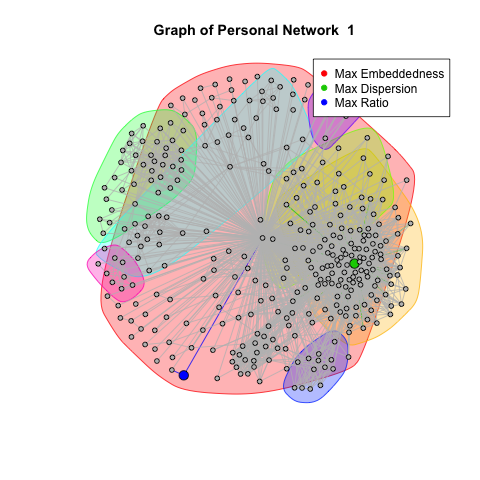
\includegraphics[scale=0.4]{d14} \\
 
 \item \textbf{Personal Network 2}\\
 The core node is node with id 108. The node with maximum embeddedness is 1889.
 The node with maximum dispersion is 1747 and the one with maximum dispersion2 is 1889.
 The node with the maximum ratio of dispersion1 to embeddedness is 1.
 The node with the maximum ratio of dispersion2 to embeddedness is 1066.\\
 \textbf{Using Dispersion 1 :}\\
 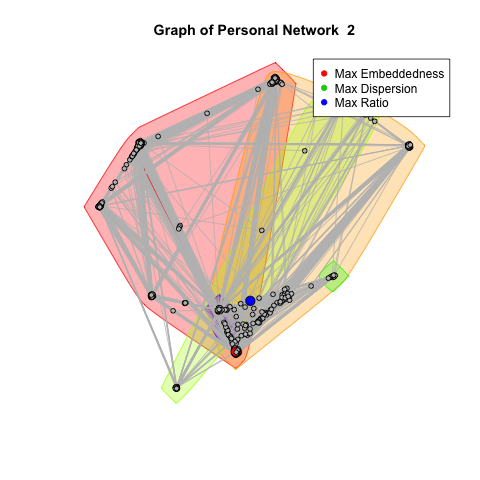
\includegraphics[scale=0.4]{d12} \\
 \textbf{Using Dispersion 2 :}\\
 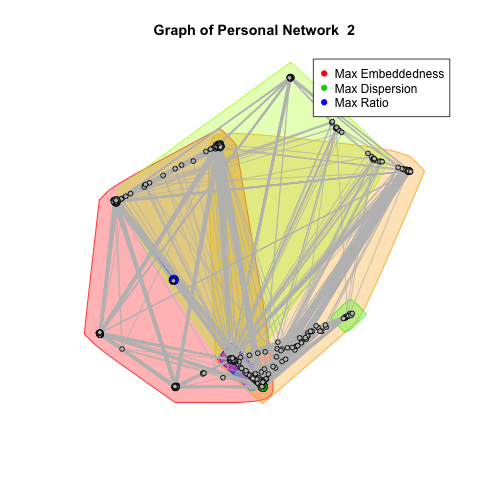
\includegraphics[scale=0.4]{d15} \\
 
 \item \textbf{Personal Network 3}\\
 The core node is node with id 349. The node with maximum embeddedness is 377.
 The node with maximum dispersion is 413 and the one with maximum dispersion2 is 377.
 The one with the maximum ratio of dispersion1 to embeddedness is 449.
 The node with the maximum ratio of dispersion2 to embeddedness  is 378.\\
 \textbf{Using Dispersion 1 :}\\
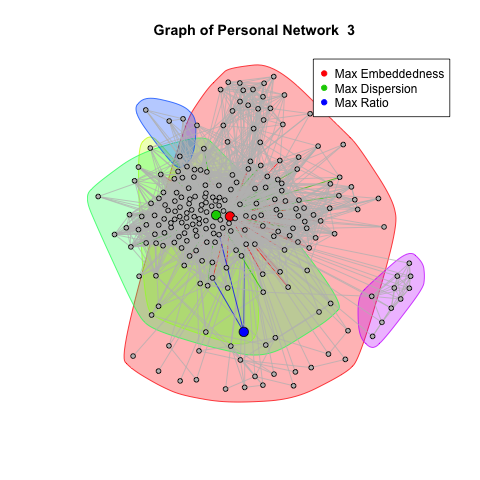
\includegraphics[scale=0.4]{d13} \\
 \textbf{Using Dispersion 2 :}\\
 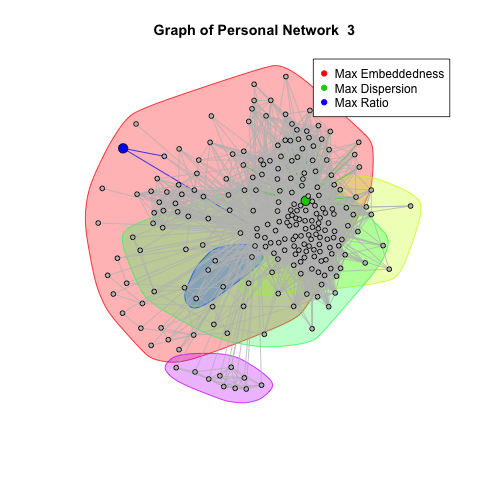
\includegraphics[scale=0.4]{d16} \\
\end{enumerate}
Curiously, we observe that for dispersion2, the node with the highest value is the same as the node with the maximum embeddeddness.
This provides some insight into this measure of distance we used.\\
Also, for both dispersions, the general trend we observe for both notions of dispersion 
is that nodes with lower dispersion by
embeddedness ratio have lower degrees.\\

To elaborate more on the characteristics of a node revealed by these measures, we observe that a node with higher
embeddeddness is a node that is very closely linked to the user whose personal network we are analyzing.
Nodes with high dispersion correspond to people who have a lot of mutual friends with that user, but the mutual friends
aren't really a close knit group. In the reference paper, this is used to identify romantic partners in a social network.
Ratio of dispersion/embeddeddness again provides very similar interpretations.

\hrule

\paragraph{Problem 6}:\\
In this question, we have to find out the similarities between communities found in the personal network of a user.
We first take personal networks of all users (40 in number) and find out the community structures between 
them using the Fast Greedy algorithm as well as the Infomap algorithm. For each community we 
calculate the following three features - size of the community, density of the community (which 
shows how densely connected the community is) and the clustering coefficient.\\

From these calculated features for all communities, we notice that density and clustering coefficient 
are correlated. So, we continue our analysis only with density and size features.\\

From the trends of these two features we notice that, for each personal network, there exists two kinds of communities:\\
\begin{itemize}
 \item \textbf{Community Type 1}\\
The community with the smallest size is also the community that has the highest density.
\item \textbf{Community Type 2}
The community with the largest size is also the community that has the lowest density.
\end{itemize}
We confirmed that
these trends are uniform across \textbf{majority(90\%)} of personal networks created by the Fast Greedy algorithm. The 
Infomap algorithm, however, does not give very conclusive results.
The interpretation of the above two communities that are common across all personal networks is that 
each personal network might have a community that represents the family of the core node. This community will be 
smaller but since it consists of family members, it will be densely connected. The reverse interpretation can be 
applied for the largest community which might just have acquaintances.\\

We have plotted the sizes and densities for both these types of communities to graphically represent this interpretation.\\
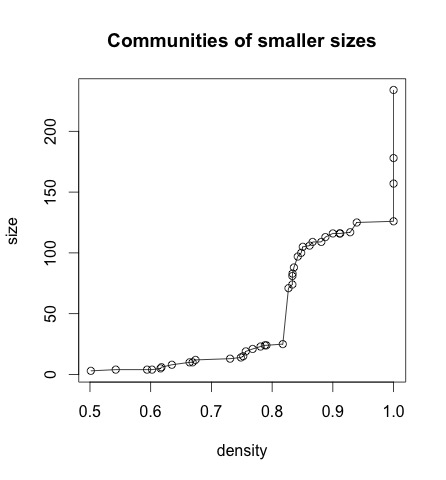
\includegraphics[scale=0.4]{Q6a} \\
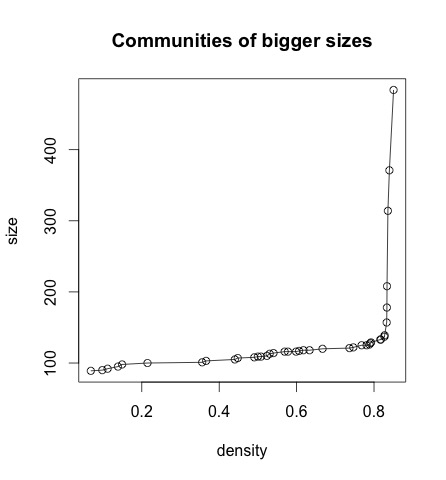
\includegraphics[scale=0.4]{Q6b} \\
\paragraph{Problem 7}:\\
We perform the same kind of analysis as in the previous questions, but on
the google+ social network. In this network, users' ``friends'' are organised in the form of circles
with the additional feature that a user $x$ can have user $y$ in his circles but the vice versa need not be true.
To analyze it abstractly, we can think of this social network as a directed graph unlike in the case of facebook where
it was a directed graph. Additionally, in google+, circles denote specific tags that users put on relationships. 
For example, a user could have a separate circle for family, one for colleagues in work, etc.\\

We first download the google+ edgelist and 
create personal networks (defined as in the previous questions) for users who have more than 2 circles. 
Since there are several such personal networks, we restrict our attention to just 5 of them and
generalize our obsercations. We extract the community structure of each personal network using two methods - 
walktrap and infomap. After this, we find out the overlap between these communities and the users' circles. Since
this overlap is not easily discernible by visually interpreting the two objects, we use certain computable features
of each of them to try to model the extent of overlap. We also try to analyse how this overlap varies across different users
and how it relates to a user's habit of tagging relationships with circles.\\

\textbf{Node 1 }\\
The id of this node is $101541879642294398860$.
The personal network of this node is shown below :\\
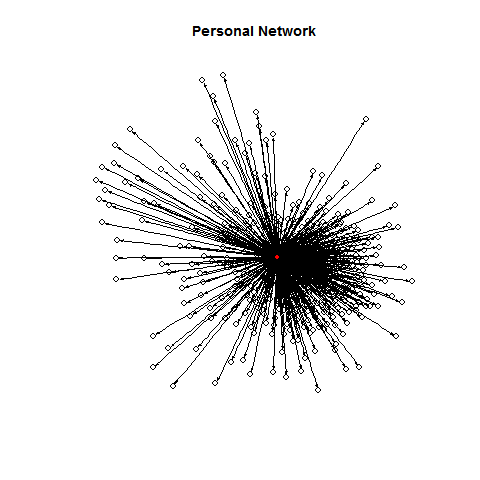
\includegraphics[scale=0.6]{7_1a} \\
The circles of the node are shown below where we color each node differently
depending on the circle it belongs to.\\
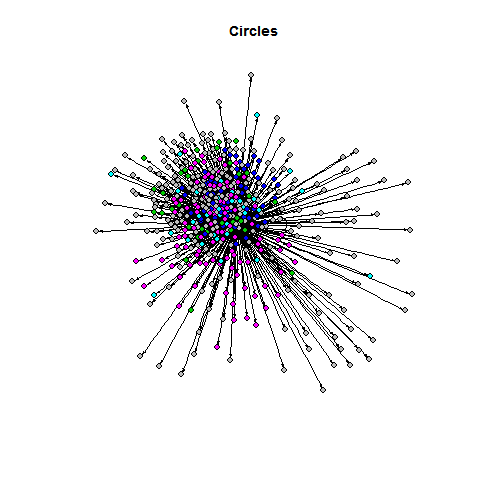
\includegraphics[scale=0.6]{7_1d} \\
The community structures are created below according to the two methods.\\
\begin{enumerate}
 \item \textbf{Infomap}\\
 We compute the community structure using the infomap algorithm.\\
 In the first plot shown below, the x-axis denotes the sizes of the communities and the y-axis has the number of communities with that size.\\
	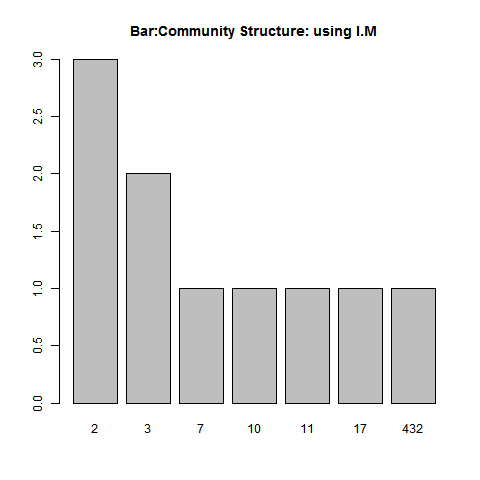
\includegraphics[scale=0.4]{7_1b} \\
	In the next plot we provide a pictorial representation of the community structure.
	We color each community differently to help distinguish between them.\\
	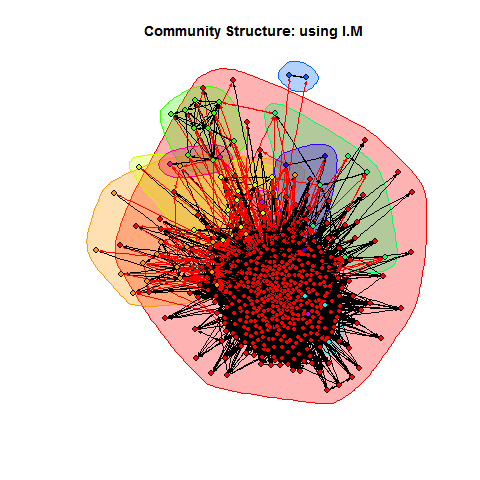
\includegraphics[scale=0.7]{7_1c} \\ 

 Now, we try to show an overlap between the two communities in the following plot.
Here, the nodes are colored on the basis of the circles in which they belong and 
the overlapped area is colored according to the community in which it belongs.\\
 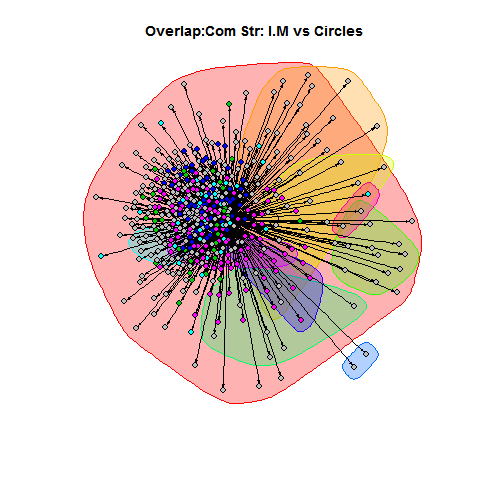
\includegraphics[scale=0.7]{7_1e} \\
 
 We also provide a quantitative measure of analyzing overlap as follows: for each circle in the network,
 we compute what percentage of its vertices is present in each community and tabulate the maximum value in that.
 Let's call this measure as the ``best fit value''. Also, here the size of the circle denotes the number of nodes in it.
\begin{table}[ht]
\caption{Overlap}
\centering
\begin{tabular}{| c | c | c |}
\hline\hline
\newline

Circle number & Size & Best Fit Value \\ [0.5ex]
\hline

1 & 90 & 0.9111 \\
\hline
2 & 92 & 0.9565 \\
\hline
3 & 93 & 0.9784 \\
\hline
4 & 48 & 0.8958 \\
\hline
5 & 105 & 0.9047 \\
\hline
\end{tabular}
\end{table} 

\item \textbf{Walktrap}\\
 We compute the community structure using the walktrap algorithm.
 In the first plot shown below, the x-axis denotes the sizes of the communities and the y-axis has the number of communities with that size.\\
	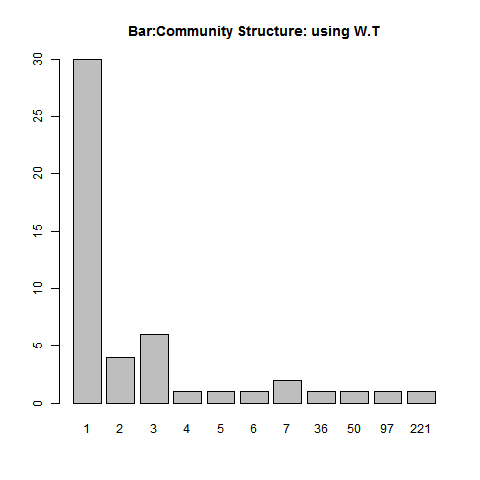
\includegraphics[scale=0.4]{7_1f} \\
	In the next plot we provide a pictorial representation of the community structure.
	We color each community differently to help distinguish between them.\\
	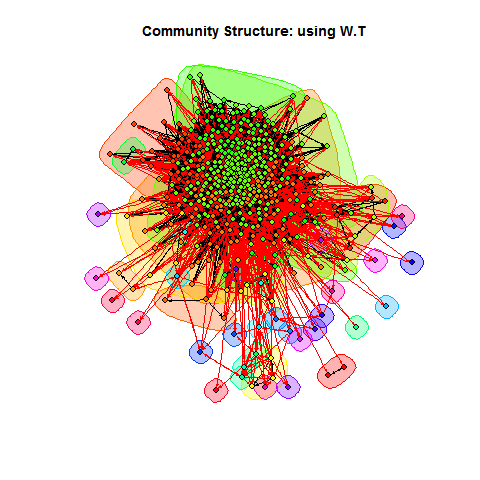
\includegraphics[scale=0.7]{7_1g} \\ 

 Now, we try to show an overlap between the two communities in the following plot.
Here, the nodes are colored on the basis of the circles in which they belong to and 
the overlapped area is colord according to the community in which it belongs.\\
 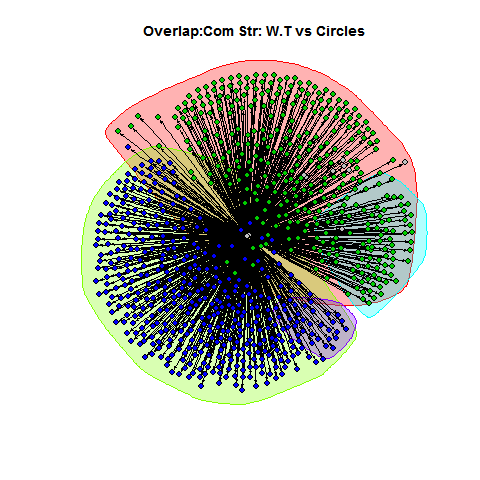
\includegraphics[scale=0.7]{7h} \\
 
 We also provide a quantitative measure of analyzing overlap as in the previous case.
\begin{table}[ht]
\caption{Overlap}
\centering
\begin{tabular}{|c |c |c |}
\hline\hline
\newline

Circle number & Size & Best Fit Value \\ [0.5ex]
\hline

1 & 90 & 0.4222 \\
\hline
2 & 92 & 0.4673 \\
\hline
3 & 93 & 0.5806 \\
\hline
4 & 48 & 0.4375 \\
\hline
5 & 105 & 0.4285 \\
\hline
\end{tabular}
\end{table} 
\end{enumerate}

\textbf{Node 2 }\\
The id of this node is $107459220492917008623$.
The personal network of this node is shown below :\\
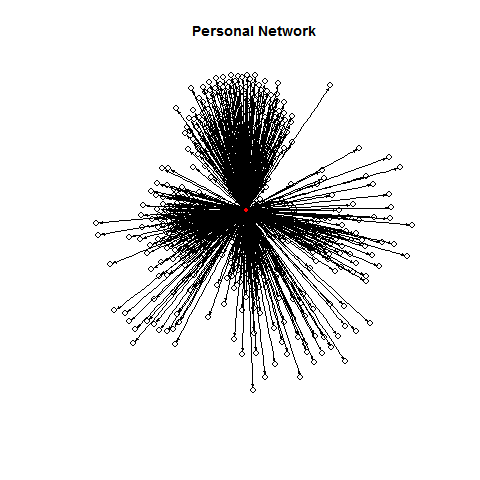
\includegraphics[scale=0.6]{7_2a} \\
The circles of the node are shown below where we color each node differently
depending on the circle it belongs to.\\
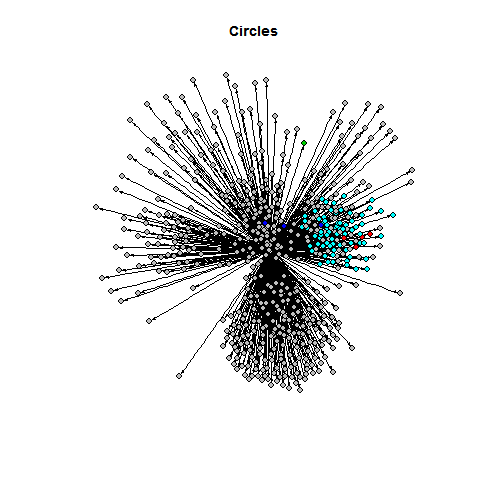
\includegraphics[scale=0.6]{7_2d} \\
The community structures are created below according to the two methods.\\
\begin{enumerate}
 \item \textbf{Infomap}\\
 We compute the community structure using the infomap algorithm.\\
 In the first plot shown below, the x-axis denotes the sizes of the communities and the y-axis has the number of communities with that size.\\
	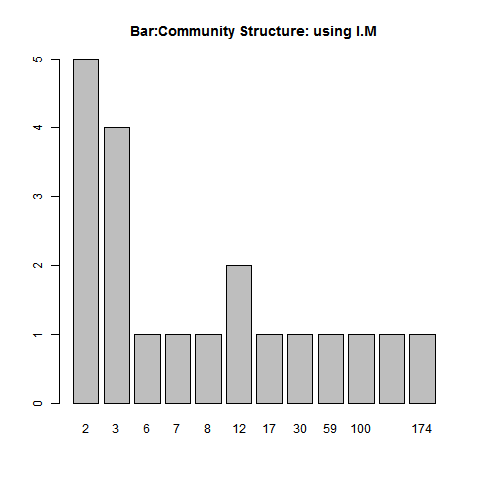
\includegraphics[scale=0.4]{7_2b} \\
	In the next plot we provide a pictorial representation of the community structure.
	We color each community differently to help distinguish between them.\\
	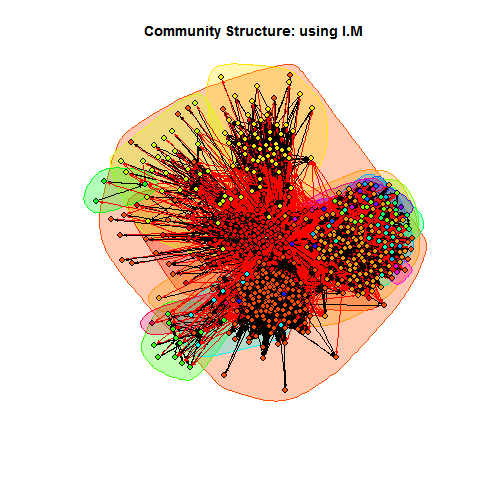
\includegraphics[scale=0.7]{7_2c} \\ 

 Now, we try to show an overlap between the two communities in the following plot.
Here, the nodes are colored on the basis of the circles in which they belong and 
the overlapped area is colored according to the community in which it belongs.\\
 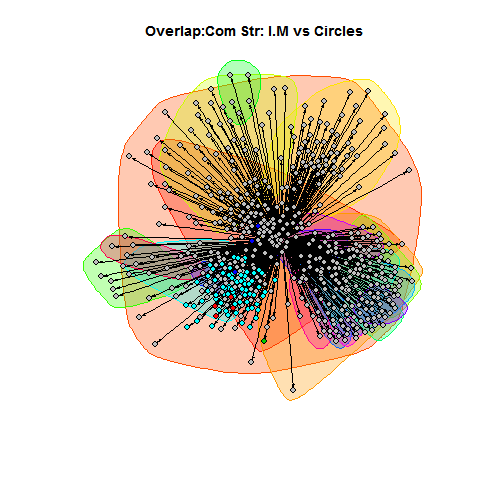
\includegraphics[scale=0.7]{7_2e} \\
 
 We also provide a quantitative measure of analyzing overlap as follows: for each circle in the network,
 we compute what percentage of its vertices is present in each community and tabulate the maximum value in that.
 Let's call this measure as the ``best fit value''. Also, here the size of the circle denotes the number of nodes in it.
\begin{table}[ht]
\caption{Overlap}
\centering
\begin{tabular}{| c | c | c |}
\hline\hline
\newline

Circle number & Size & Best Fit Value \\ [0.5ex]
\hline

1 & 5 & 0.8 \\
\hline
2 & 5 & 0.8 \\
\hline
3 & 5 & 0.4 \\
\hline
4 & 71 & 0.9577 \\
\hline
\end{tabular}
\end{table} 

\item \textbf{Walktrap}\\
 We compute the community structure using the walktrap algorithm.
 In the first plot shown below, the x-axis denotes the sizes of the communities and the y-axis has the number of communities with that size.\\
	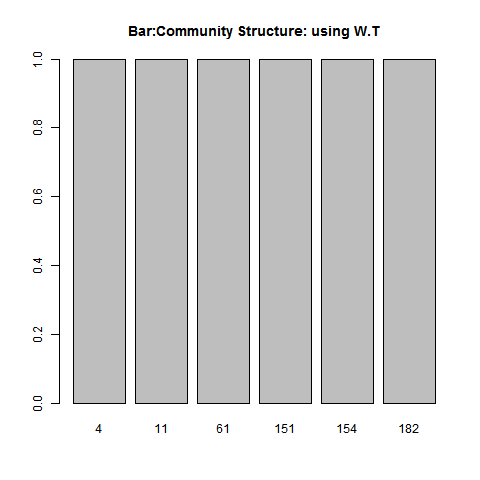
\includegraphics[scale=0.4]{7_2f} \\
	In the next plot we provide a pictorial representation of the community structure.
	We color each community differently to help distinguish between them.\\
	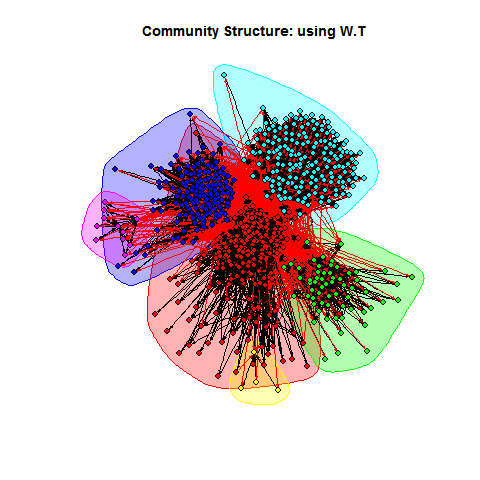
\includegraphics[scale=0.7]{7_2g} \\ 

 Now, we try to show an overlap between the two communities in the following plot.
Here, the nodes are colored on the basis of the circles in which they belong to and 
the overlapped area is colord according to the community in which it belongs.\\
 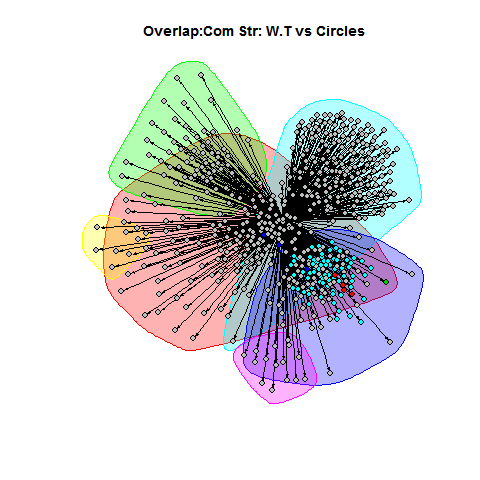
\includegraphics[scale=0.7]{7_2h} \\
 
 We also provide a quantitative measure of analyzing overlap as in the previous case.
\begin{table}[ht]
\caption{Overlap}
\centering
\begin{tabular}{|c |c |c |}
\hline\hline
\newline

Circle number & Size & Best Fit Value \\ [0.5ex]
\hline
1 & 5 & 0.8 \\
\hline
2 & 5 & 0.8 \\
\hline
3 & 5 & 0.4 \\
\hline
4 & 71 & 0.9859 \\
\hline

\end{tabular}
\end{table} 
\end{enumerate}

\textbf{Node 3 }\\
The id of this node is $109327480479767108490$.
The personal network of this node is shown below :\\
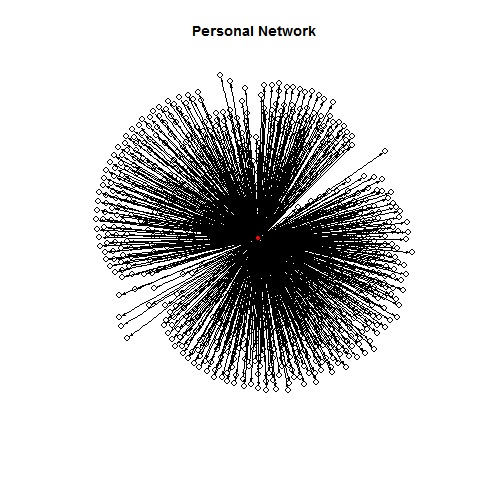
\includegraphics[scale=0.6]{7a} \\
The circles of the node are shown below where we color each node differently
depending on the circle it belongs to.\\
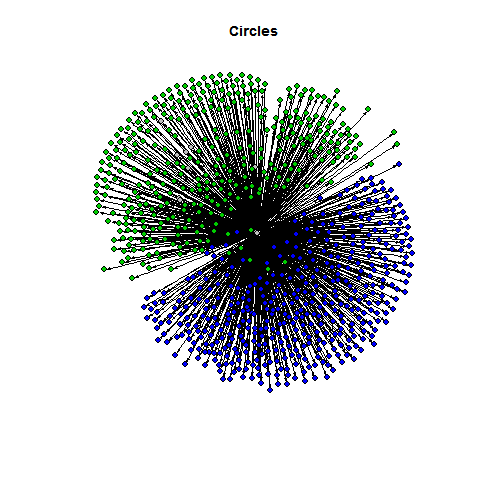
\includegraphics[scale=0.6]{7d} \\
The community structures are created below according to the two methods.\\
\begin{enumerate}
 \item \textbf{Infomap}\\
 We compute the community structure using the infomap algorithm.\\
 In the first plot shown below, the x-axis denotes the sizes of the communities and the y-axis has the number of communities with that size.\\
	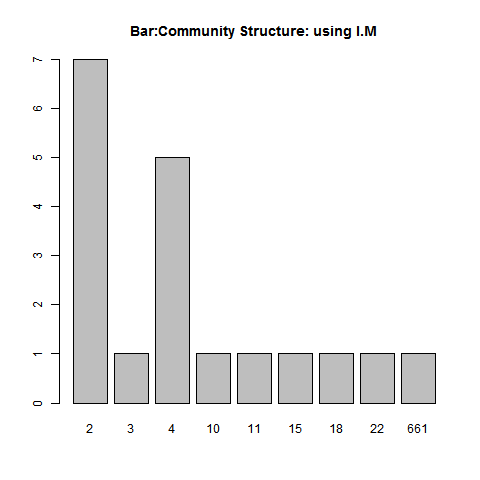
\includegraphics[scale=0.4]{7b} \\
	In the next plot we provide a pictorial representation of the community structure.
	We color each community differently to help distinguish between them.\\
	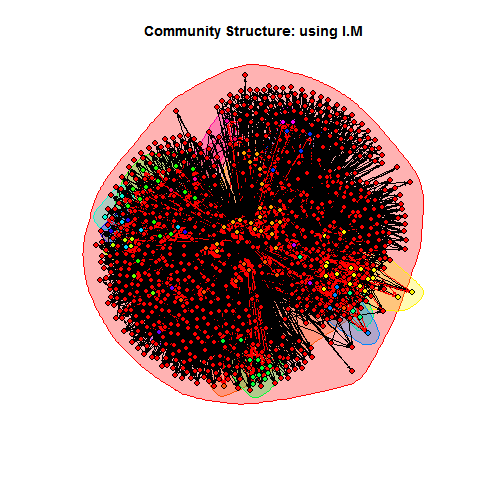
\includegraphics[scale=0.7]{7c} \\ 

 Now, we try to show an overlap between the two communities in the following plot.
Here, the nodes are colored on the basis of the circles in which they belong and 
the overlapped area is colored according to the community in which it belongs.\\
 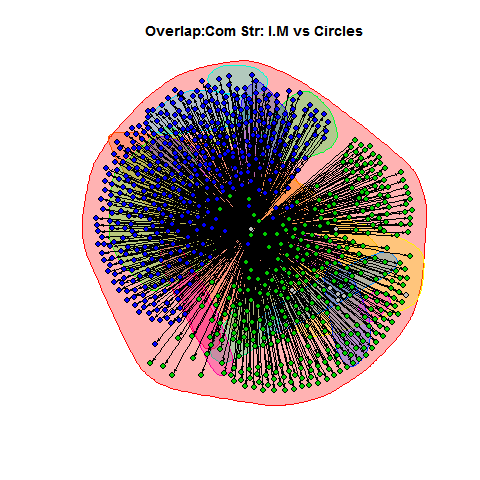
\includegraphics[scale=0.7]{7e} \\
 
 We also provide a quantitative measure of analyzing overlap as follows: for each circle in the network,
 we compute what percentage of its vertices is present in each community and tabulate the maximum value in that.
 Let's call this measure as the ``best fit value''. Also, here the size of the circle denotes the number of nodes in it.
\begin{table}[ht]
\caption{Overlap}
\centering
\begin{tabular}{| c | c | c |}
\hline\hline
\newline

Circle number & Size & Best Fit Value \\ [0.5ex]
\hline

1 & 331 & 0.8489 \\
\hline
2 & 347 & 0.8530 \\
\hline
3 & 420 & 0.8666 \\
\hline
\end{tabular}
\end{table} 

\item \textbf{Walktrap}\\
 We compute the community structure using the walktrap algorithm.
 In the first plot shown below, the x-axis denotes the sizes of the communities and the y-axis has the number of communities with that size.\\
	\includegraphics[scale=0.4]{7f} \\
	In the next plot we provide a pictorial representation of the community structure.
	We color each community differently to help distinguish between them.\\
	\includegraphics[scale=0.7]{7g} \\ 

 Now, we try to show an overlap between the two communities in the following plot.
Here, the nodes are colored on the basis of the circles in which they belong to and 
the overlapped area is colord according to the community in which it belongs.\\
 \includegraphics[scale=0.7]{7h} \\
 
 We also provide a quantitative measure of analyzing overlap as in the previous case.
\begin{table}[ht]
\caption{Overlap}
\centering
\begin{tabular}{|c |c |c |}
\hline\hline
\newline

Circle number & Size & Best Fit Value \\ [0.5ex]
\hline

1 & 331 & 0.7583 \\
\hline
2 & 347 & 0.7694 \\
\hline
3 & 420 & 0.9357 \\
\hline
\end{tabular}
\end{table} 
\end{enumerate}

\textbf{Observations:}\\
We observe a common trend in all the personal networks that as the size of the circle increases, the best fit value increases.
This shows that the amount of overlap of the circle with the communities increases as the size of the circle increases.
This follows along expected lines and hence gives more belief that our notion of 
``best fit value'' does indeed capture the overlap between circles and communities.
We also notice that in the case of the first node, the best fit value (and hence the overlap) is much higher when the communities
are calculated using the infomap method than in the case of the walktrap method. In the other two nodes, the results are quite similar.
We can extrapolate this to suggest that, in general, the infomap algorithm works better to capture the overlap with circles.

\end{document}
